\documentclass[12pt, a4paper]{article}

\usepackage[utf8]{inputenc}
\usepackage[vietnamese]{babel}
\usepackage{fontspec}
\setmainfont{Times New Roman}

\usepackage{graphicx}
\usepackage{amsmath, amssymb, amsfonts}
\usepackage{hyperref}
\hypersetup{
    colorlinks=true,
    linkcolor=blue,
    citecolor=black,
    urlcolor=blue
}

\usepackage{tikz}
\usetikzlibrary{calc}

\usepackage[left=3cm, right=2cm, top=2cm, bottom=2cm]{geometry}

\usepackage{fancyhdr}
\pagestyle{fancy}
\fancyhf{}

\fancyhead[L]{\textbf{Cấu trúc dữ liệu và giải thuật nâng cao}}
\fancyhead[R]{\textbf{TÀI LIỆU GIỚI THIỆU ỨNG DỤNG QUẢN LÝ SINH VIÊN}}
\fancyhead[L]{\textbf{Cấu trúc dữ liệu và giải thuật nâng cao}}
\fancyhead[R]{\textbf{ỨNG DỤNG QUẢN LÝ SINH VIÊN}}
\fancyfoot[C]{\thepage}

\setcounter{secnumdepth}{3} 
\setcounter{tocdepth}{3}    

\renewcommand{\thesection}{\arabic{section}.}
\renewcommand{\thesubsection}{\arabic{section}.\arabic{subsection}.}
\renewcommand{\thesubsubsection}{\arabic{section}.\arabic{subsection}.\arabic{subsubsection}.}

\usepackage{tocloft}

\renewcommand{\cfttoctitlefont}{\hfill\fontsize{24}{24}\selectfont\bfseries}
\renewcommand{\cftaftertoctitle}{\hfill}

\setlength{\cftbeforetoctitleskip}{10pt} % Khoảng cách phía trên
\setlength{\cftaftertoctitleskip}{30pt}  % Khoảng cách phía dưới (cách các mục lục bên dưới)

\begin{document}

% titlepage.tex
\begin{titlepage}
    \newgeometry{left=2cm, right=2cm, top=2cm, bottom=2cm}
    \thispagestyle{empty} 
    
    \begin{tikzpicture}[overlay, remember picture]
        \draw [line width=3pt, draw=blue] ($(current page.north west) + (1.2cm,-1.0cm)$) 
            rectangle ($(current page.south east) + (-1.0cm,1.5cm)$);
        \draw [line width=0.5pt, draw=blue] ($(current page.north west) + (1.3cm,-1.1cm)$) 
            rectangle ($(current page.south east) + (-1.1cm,1.6cm)$);
    \end{tikzpicture}

    \begin{center}
        {\fontsize{17}{14}\selectfont \textbf{ĐẠI HỌC QUỐC GIA THÀNH PHỐ HỒ CHÍ MINH}} \\
        {\fontsize{17}{14}\selectfont \textbf{TRƯỜNG ĐẠI HỌC CÔNG NGHỆ THÔNG TIN}} \\
        {\fontsize{18}{14}\selectfont \textbf{KHOA KHOA HỌC MÁY TÍNH}} \\
        
        \vspace{3.5cm}
        
        \IfFileExists{images/UIT_logo.png}{
            
\includegraphics[width=8cm]{images/UIT_logo.png}
        }{
            \vspace{2.5cm} 
        }
        
        \vspace{2.5cm}
        
        {\fontsize{20}{16}\selectfont \textbf{CẤU TRÚC DỮ LIỆU VÀ GIẢI THUẬT NÂNG CAO}}\\
        {\fontsize{20}{24}\selectfont \textbf{TÀI LIỆU GIỚI THIỆU}} \\
        {\fontsize{20}{24}\selectfont \textbf{ỨNG DỤNG QUẢN LÝ SINH VIÊN}} \\
        
        \vspace{2.5cm}
        
        \begin{minipage}{0.8\textwidth}
            \begin{tabular}{ll}
                \fontsize{17}{16}\textbf{Giảng viên hướng dẫn:} & \fontsize{16}{16}\textbf{Nguyễn Thanh Sơn} \\ 
                \fontsize{17}{16}\textbf{Sinh viên thực hiện:} & \fontsize{16}{16}\textbf{24521344 - Thái Hoàng Huy Phong} \\
            \end{tabular}
        \end{minipage}
        
        \vfill
        {\fontsize{18}{14}\selectfont \textbf{THÀNH PHỐ HỒ CHÍ MINH, 2026}}
    \end{center}
    
    \restoregeometry 
\end{titlepage}

\newpage
\tableofcontents
\newpage

\section{Giới thiệu tổng quan}
\indent Hệ thống Quản lý Sinh viên là một ứng dụng web trực quan
được thiết kế nhằm mục đích mô phỏng và ứng dụng cấu trúc dữ liệu Cây B-Tree  vào thực tế.

\indent Thay vì sử dụng các hệ quản trị cơ sở dữ liệu có sẵn, 
dự án này tự xây dựng một hệ thống lưu trữ tệp nhị phân kết hợp với thuật toán lập chỉ mục bằng B-Tree để
tối ưu hóa tốc độ tìm kiếm, thêm và xóa dữ liệu.

Mã nguồn chi tiết và chương trình demo cài đặt B-Tree được lưu trữ công khai. 
Truy cập tại đây:
\begin{itemize}
    \item \href{https://github.com/146huyphong/Simulation-Database}{Source Code Demo trên GitHub}: https://github.com/146huyphong/Simulation-Database
    \item \href{https://leafy-liger-fd5843.netlify.app/}{Demo trực tuyến}: https://leafy-liger-fd5843.netlify.app
\end{itemize}

Các công nghệ sử dụng:
\begin{itemize}
    \item Giao diện: HTML5, CSS3, JavaScript (É6+)
    \item Vẽ biểu đồ: Thư viện D3.js
    \item Máy chủ: Python3, Flask, Flask-CORS
    \item Lưu trữ dữ liệu: Tệp nhị phân (student.dat)
\end{itemize}

\section{Tính năng nổi bật}
\begin{itemize}
    \item \textbf{Lập chỉ mục kép}: Hệ thống duy trì song song hai cây B-Tree: một cây sắp xếp theo Mã số sinh viên và một cây sắp xếp theo Họ Tên,
    giúp tối ưu hóa đa dạng các loại truy vấn.
    \item \textbf{Mô phỏng trực quan}: Bất kỳ thay đổi nào về dữ liệu (Thêm/Xóa) đều được minh họa ngay lập tức lên biểu đồ cây B-Tree bằng D3.js.
    \item \textbf{Kiến trúc tách biệt}: Hệ thống giao tiếp hoàn toàn qua RESTful API, cho phép triển khai Frontend và Backend trên các máy chủ đám mây hoàn toàn khác nhau. 
\end{itemize} 

\section{Hướng dẫn sử dụng hệ thống}
\indent Để sử dụng hệ thống, người dùng cần thực hiện các bước sau:
\subsection{Thêm mới sinh viên}
\begin{itemize}
    \begin{figure}[H]
        \centering
        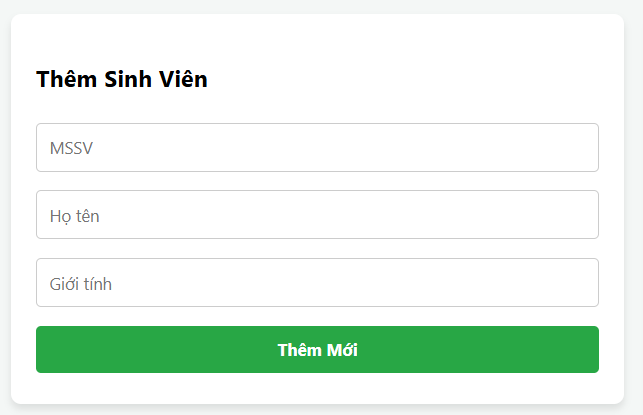
\includegraphics[width=0.8\textwidth]{images/description/insert_border.png}
        \caption{Khu vực thêm sinh viên}
    \end{figure}
    \item Bước 1: Tại khu vực ``Thêm Sinh Viên Mới'' đầy đủ thông tin vào các ô: Mã SV, Họ Tên và Giới tính.
    \item Bước 2: Nhấn nút Thêm Sinh Viên.
\end{itemize}

\begin{figure}[H]
    \centering
    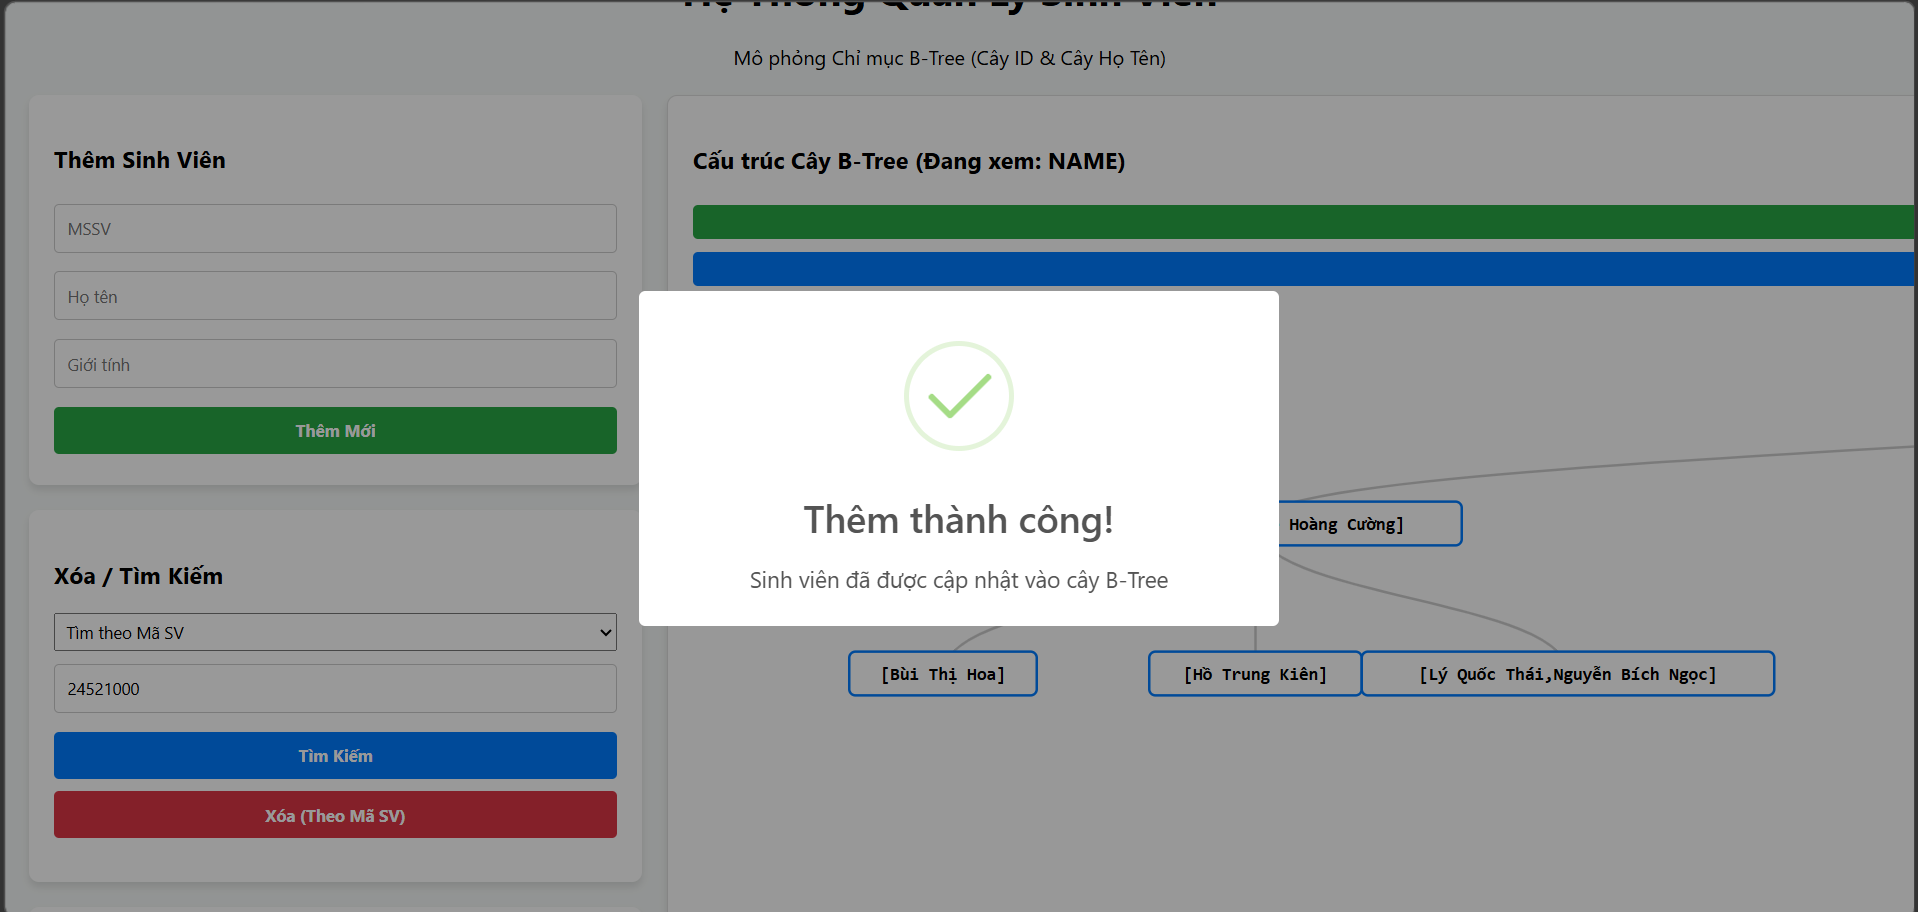
\includegraphics[width=0.8\textwidth]{images/description/result_insert.png}
    \caption{Kết quả khi thêm mới thành công}
\end{figure}
Kết quả: Hệ thống sẽ lưu dữ liệu vào file nhị phân. Bảng danh sách bên dưới và cấu trúc cây B-Tree bên phải sẽ tự động giật load và vẽ lại ngay lập tức để hiển thị node mới được chèn vào.

\subsection{Xóa sinh viên}
\begin{itemize}
    \begin{figure}[H]
        \centering
        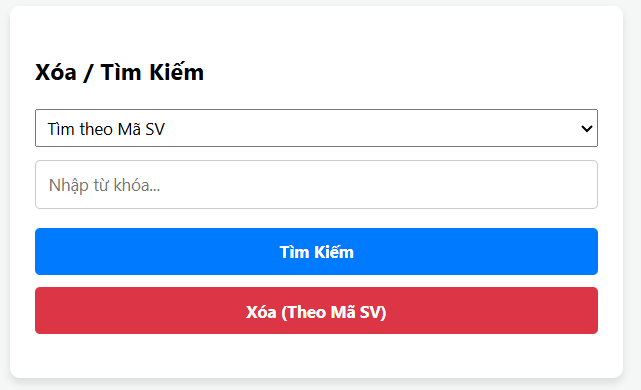
\includegraphics[width=0.8\textwidth]{images/description/search_delete_border.png}
        \caption{Khu vực tìm kiếm/xóa sinh viên}
    \end{figure}
    \item Bước 1: Tại khu vực ``Tìm kiếm/Xóa (Theo Mã SV)'', chọn tiêu chí tìm kiếm ở menu thả xuống: Xóa theo Mã SV hoặc Họ Tên.
    \item Bước 2: Nhập chính xác Mã số sinh viên của sinh viên cần xóa
    \item Bước 3: Nhấn nút \textbf{Xóa}
\end{itemize}
    \begin{figure}[H]
        \centering
        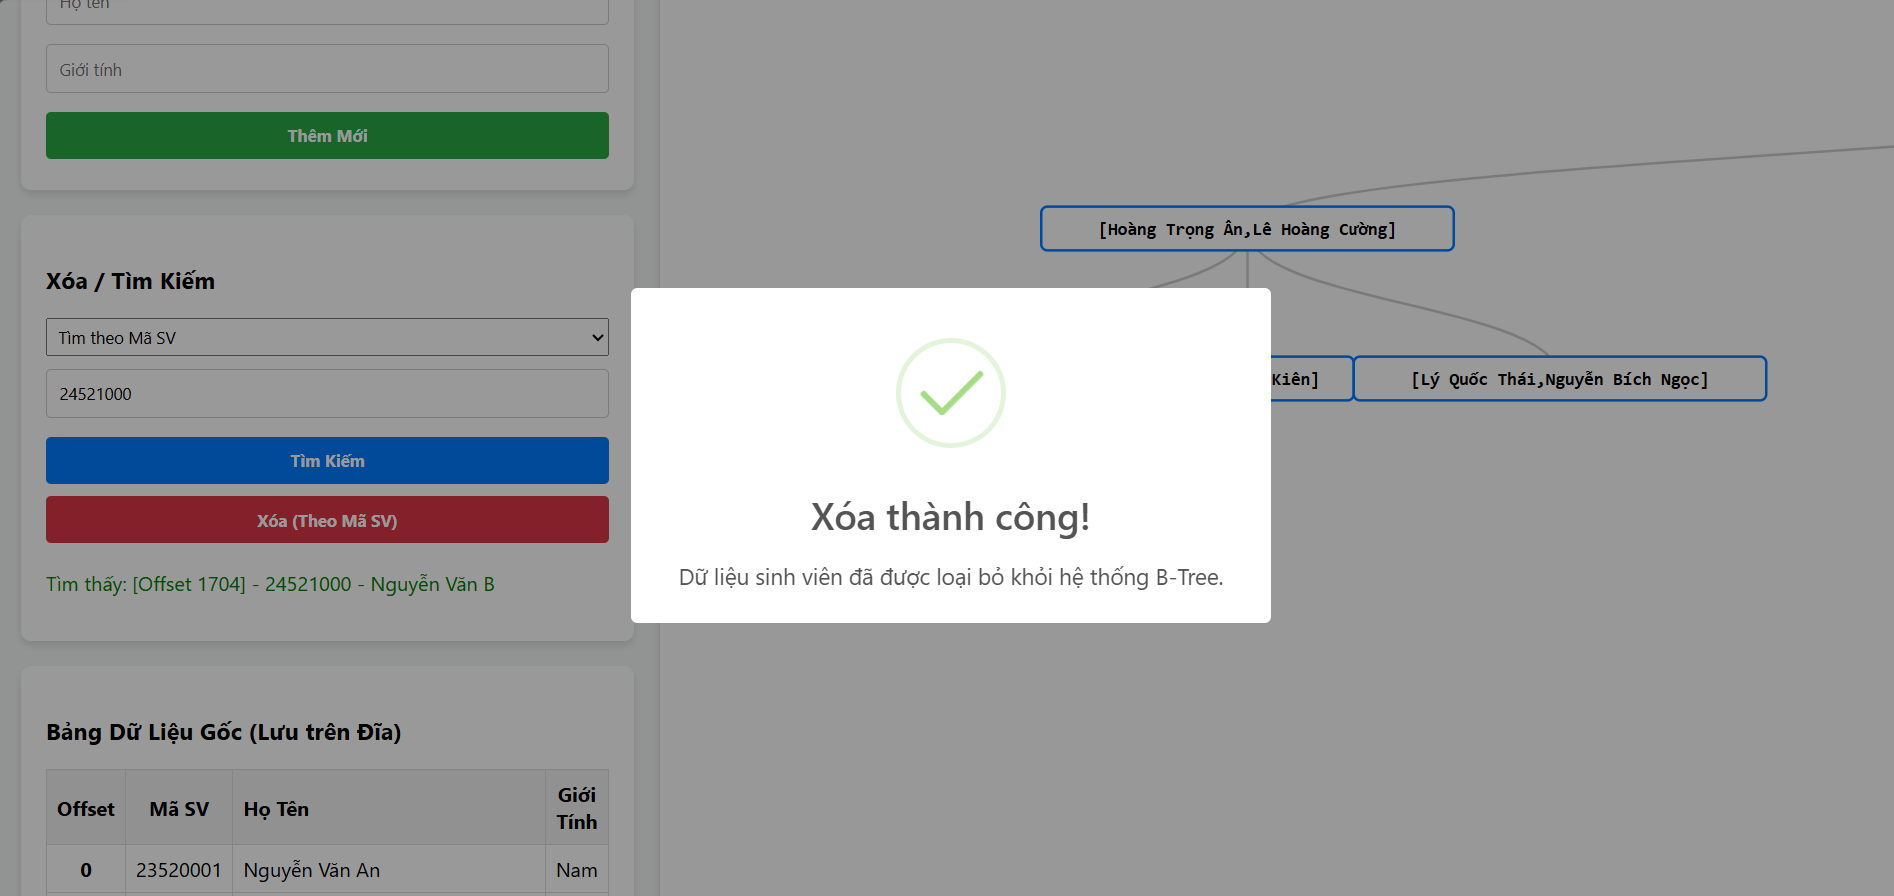
\includegraphics[width=0.8\textwidth]{images/description/result_delete.png}
        \caption{Kết quả khi xóa thành công}
    \end{figure}
Kết quả: Dữ liệu sẽ bị đánh dấu xóa trong file nhị phân. Node tương ứng trên cây B-Tree sẽ biến mất và cây sẽ tự động cân bằng lại theo đúng thuật toán B-Tree.

\subsection{Tìm kiếm sinh viên}
\begin{itemize}
    \item Bước 1: Tại khu vực ``Tìm kiếm / Xóa'', chọn tiêu chí tìm kiếm ở menu thả xuống: Tìm theo Mã SV hoặc Họ Tên.
    \item Bước 2: Nhập từ khóa tương ứng vào ô nhập liệu.
    \item Bước 3: Nhấn nút Tìm kiếm.
\end{itemize}

\begin{figure}[H]
    \centering
    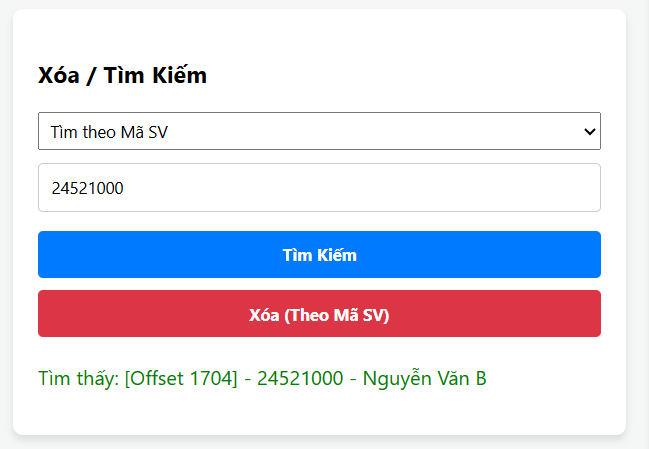
\includegraphics[width=0.8\textwidth]{images/description/search_result.png}
    \caption{Kết quả tìm kiếm sinh viên tồn tại}
\end{figure}
Kết quả: Bảng thông báo bên dưới sẽ hiển thị thông tin sinh viên tìm được, kèm theo địa chỉ Offset.

\subsection{Tương tác với Biểu đồ Cây B-Tree}
\begin{itemize}
    \item Chuyển đổi góc nhìn: Nhấn vào nút Cây theo ID hoặc Cây theo Tên để quan sát sự khác biệt về cấu trúc khi B-Tree sử dụng các khóa khác nhau để sắp xếp.
    \item Xem cây cỡ lớn: Khi số lượng sinh viên nhiều, cây B-Tree sẽ tự động mở rộng không gian theo chiều ngang. Bạn có thể sử dụng thanh cuộn ngang ở dưới cùng khu vực biểu đồ để kéo qua lại và quan sát toàn bộ các lá của cây một cách rõ nét, không bị chồng chéo chữ.
\end{itemize}


\end{document}